\documentclass[border=60pt, multi, tikz]{standalone}
\usepackage{import}
\subimport{../}{init}
\usetikzlibrary{positioning,fit,backgrounds,calc}
\usetikzlibrary{3d}

\def\ConvColor{rgb:yellow,5;red,2.5;white,5}
\def\ConvReluColor{rgb:yellow,5;red,5;white,5}
\def\PoolColor{rgb:red,1;black,0.3}
\def\UpSampleConvColor{rgb:blue,6;green,0.7;black,0.4}
\def\EnvelopeColor{rgb:black,1.5;white,8;blue,0.8}

\begin{document}
\begin{tikzpicture}

\tikzstyle{connection}=[ultra thick,every node/.style={sloped,allow upside down},draw=\edgecolor,opacity=0.7]

% mel spectrogram input
\node[canvas is zy plane at x=0, anchor=center] (img-in) at (-3.4,0,0) {
        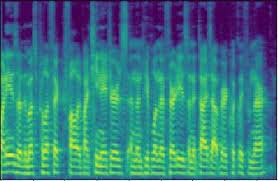
\includegraphics[width=8cm,height=8cm]{../images/sample-mel-spectrogram}
};
% Create a center point for the input image for better arrow placement
\coordinate (img-in_center) at ($(img-in)+(0.7,0,0)$);

% conv1
\pic[shift={(0,0,0)}] at (0,0,0) {RightBandedBox={name=c1,caption=Conv 1,
        xlabel={{"8","8"}},zlabel=32,fill=\ConvColor,bandfill=\ConvReluColor,
        height=40,width={2,2},depth=40}};
% pool1
\pic[shift={(1.4,0,0)}] at (c1-east) {Box={name=p1,
        xlabel=8,fill=\PoolColor,opacity=0.5,height=23,width=2,depth=23}};

% conv2
\pic[shift={(0,0,0)}] at (p1-east) {RightBandedBox={name=c2,caption=Conv 2,
        xlabel={{"16","16"}},zlabel=16,fill=\ConvColor,bandfill=\ConvReluColor,
        height=23,width={7,7},depth=23}};

% pool2
\pic[shift={(1.4,0,0)}] at (c2-east) {Box={name=p2,
        xlabel={{"16","dummy"}},fill=\PoolColor,opacity=0.5,height=10,width=7,depth=10}};

% conv3
\pic[shift={(0,0,0)}] at (p2-east) {RightBandedBox={name=c3,caption=Conv 3,
        xlabel={{"32","32"}},zlabel=8,fill=\ConvColor,bandfill=\ConvReluColor,
        height=10,width={10,10},depth=10}};

% pool3
\pic[shift={(1.4,0,0)}] at (c3-east) {Box={name=p3,caption=Conv 4,
        xlabel={{"32","dummy"}},fill=\PoolColor,opacity=0.5,height=10,width=12,depth=10}};

% conv4
\pic[shift={(0,0,0)}] at (p3-east) {RightBandedBox={name=c4,
        xlabel={{"4","4"}},zlabel=4,fill=\ConvColor,bandfill=\ConvReluColor,
        height=10,width={2,2},depth=10}};

% Encoder Envelope
\begin{scope}[on background layer]
        \pic[shift={(-0.4,0,0)}, overlay] at (c1-west) {Box={name=encoder-env,caption=Encoder,
            xlabel={{"","dummy"}},fill=\EnvelopeColor,opacity=0.2,
            height=54,width=90,depth=44}};
\end{scope}

% conv5
\pic[shift={(1.4,0,0)}] at (c4-east) {RightBandedBox={name=ci5,
        xlabel=4,fill=\ConvColor,bandfill=\ConvReluColor,
        height=10,width=2,depth=10}};
\pic[shift={(0,0,0)}] at (ci5-east) {Box={name=c5,caption=Conv 5,
        xlabel={{"4","dummy"}},fill=\ConvColor,opacity=0.5,height=10,width=16,depth=10}};
\pic[shift={(0,0,0)}] at (c5-east) {Box={name=c5b,
        xlabel={{"4","dummy"}},zlabel=4,fill=\ConvReluColor,opacity=0.5,height=10,width=7,depth=10}};

% conv6
\pic[shift={(1.4,0,0)}] at (c5b-east) {Box={name=c6,
        xlabel={{"32","dummy"}},fill=\UpSampleConvColor,
        height=10,width=10,depth=10}};
\pic[shift={(0,0,0)}] at (c6-east) {RightBandedBox={name=c6b,caption=Conv 6,
        xlabel={{"32","dummy"}},fill=\ConvColor,bandfill=\ConvReluColor,
        height=10,width=10,depth=10}};
\pic[shift={(0,0,0)}] at (c6b-east) {RightBandedBox={name=c6c,
        xlabel={{"16","dummy"}},zlabel=8,fill=\ConvColor,bandfill=\ConvReluColor,
        height=10,width={7},depth=10}};

% conv7
\pic[shift={(1.4,0,0)}] at (c6c-east) {Box={name=ci7,
        xlabel={{"16","dummy"}},fill=\UpSampleConvColor,
        height=23,width=7,depth=23}};
\pic[shift={(0,0,0)}] at (ci7-east) {RightBandedBox={name=c7,caption=Conv 7,
        xlabel={{"16","dummy"}},fill=\ConvColor,bandfill=\ConvReluColor,
        height=23,width={7},depth=23}};
\pic[shift={(0,0,0)}] at (c7-east) {RightBandedBox={name=c7b,
        xlabel=8,zlabel=16,fill=\ConvColor,bandfill=\ConvReluColor,
        height=23,width={2},depth=23}};

% conv8
\pic[shift={(1.4,0,0)}] at (c7b-east) {Box={name=ci8,
        xlabel=8,fill=\UpSampleConvColor,
        height=40,width=2,depth=40}};
\pic[shift={(0,0,0)}] at (ci8-east) {RightBandedBox={name=c8,caption=Conv 8,
        xlabel=1,zlabel=32,fill=\ConvColor,bandfill=\ConvReluColor,
        height=40,width={2},depth=40}};
\pic[shift={(1,0,0)}] at (c8-east) {RightBandedBox={name=c8b,
        xlabel=1,zlabel=32,fill=\ConvColor,bandfill=\ConvReluColor,
        height=40,width={1},depth=40}};

% Decoder Envelope
\begin{scope}[on background layer]
        \pic[shift={(0.4,0,0)}, overlay] at (ci5-west) {Box={name=encoder-env,caption=Decoder,
            xlabel={{"","dummy"}},fill=\EnvelopeColor,opacity=0.2,
            height=54,width=102,depth=44}};
\end{scope}

% mel spectrogram output
\node[canvas is zy plane at x=0, anchor=center] (img-out) at ($(c8b-east)+(3.4,0,0)$) {
        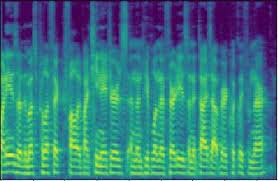
\includegraphics[width=8cm,height=8cm]{../images/sample-mel-spectrogram}
};
% Create a center point for the output image for better arrow placement
\coordinate (img-out_center) at ($(img-out)+(-0.7,0,0)$);

% Connections
\draw [connection]  (img-in_center)  -- node {\midarrow} (c1-west);
\draw [connection]  (c1-east)    -- node {\midarrow} (p1-west);
\draw [connection]  (c2-east)    -- node {\midarrow} (p2-west);
\draw [connection]  (c3-east)    -- node {\midarrow} (p3-west);
\draw [connection]  (c4-east)    -- node {\midarrow} (ci5-west);
\draw [connection]  (c5b-east)    -- node {\midarrow} (c6-west);
\draw [connection]  (c6c-east)    -- node {\midarrow} (ci7-west);
\draw [connection]  (c7b-east)    -- node {\midarrow} (ci8-west);
\draw [connection]  (c8b-east)    -- node {\midarrow} (img-out_center);

\end{tikzpicture}
\end{document}
